\documentclass{article}
\usepackage{graphicx} % Required for inserting images
\usepackage[
% backend=biber,
style=numeric, % alphabetic, numeric
natbib=true,
% maxnames=1,
% sorting=ynt
]{biblatex}
\AtEveryBibitem{
    \clearfield{urlyear}
    \clearfield{urlmonth}
}
\usepackage{hyperref}
\usepackage{xcolor}
\usepackage{amssymb}
\usepackage{amsmath}
\usepackage{wrapfig}
\usepackage{multirow}  % tables double entry
\usepackage{geometry}
\usepackage{bbm}  % makes mathbbm{1} vector 1
\usepackage{cleveref}
\usepackage{algorithm}
\usepackage{algpseudocode}
\usepackage{parskip}
\usepackage{amsthm}
% tables
\usepackage{booktabs}
\usepackage{tabularx} % For text wrapping in the last column
\usepackage{multirow} % Required to span cells across rows
\usepackage[title]{appendix} % Generates "Appendix A" instead of just "A"

% for definitions
\theoremstyle{definition}
\newtheorem{definition}{Definition}[section]
\newtheorem{example}{Example}[section]
\theoremstyle{remark}
\newtheorem*{remark}{Remark}
\newtheoremstyle{resultstyle}% name of the style to be used
  {10pt}% measure of space to leave above the theorem. E.g.: 3pt
  {\topsep}% measure of space to leave below the theorem. E.g.: 3pt
  {\itshape}% name of font to use in the body of the theorem
  {0pt}% measure of space to indent
  {\bfseries}% name of head font
  {. ---}% punctuation between head and body
  { }% space after theorem head; " " = normal interword space
  {\thmname{#1}\thmnumber{ #2}\textnormal{\thmnote{ (#3)}}}
\theoremstyle{resultstyle}
\newtheorem{theorem}{Theorem}[section]
\newtheorem{proposition}{Proposition}[section]
\newtheorem{conjecture}{Conjecture}[section]
\newtheorem{corollary}{Corollary}[section]
\newtheorem{lemma}{Lemma}[section]

\geometry{margin=1in}
% \setlength\parindent{10pt}  % Paragraph indentation
\newcommand{\pnote}[1]{\textcolor{red}{PL: #1}}
\newcommand{\myline}{%
  \vspace{5mm}%
  \hrule%
  \vspace{5mm}%
}

\addbibresource{references.bib} %Import the bibliography file

\title{Symmetries and Deep Learning: a Survey}
\author{Pierrick Leroy}
\date{2026}

\begin{document}

\maketitle

\begin{abstract}
% Audience: reader curious to know about occurences of symmetries in a deep learning context

\pnote{write at the end}

\end{abstract}

\section{Introduction}

\pnote{write at the end}



\newpage
\begin{appendices}
% Reset table numbering to A.1, A.2, etc. per section
\counterwithin{table}{section}

\section{Group table}

\end{appendices}

\printbibliography

% \section*{Draft}

\myline

\paragraph{Neural surrogates}
% should PINNs be considered in the survey ?
Physics informed neural networks \citep{raissi2019jocp} combine data-driven machine learning with priors about the physical laws known to apply to the system.
Many applications such as fluid motion or wave propagation rely on the time-translation invariance of physical laws.

\myline

\paragraph{Language symmetries}
% huang2021p2cnacaclhlt, krishna2020p2cemnlpe, yamshchikov2021pacai, bianchi2022pnpfwebn, zarza2026, gordon2020

\myline

\cite{pertigkiozoglou2024} train non strictly equivariant model and converge to a strictly equivariant one, easing the optimization.

\myline

In parallel, \cite{kondor2018,thomas2018} create equivariant architecture working directly in the Fourier space.

\myline

\paragraph{Steerable CNNs}
\cite{weiler2019anips} studies general $E(2)$-equivariant CNNs, using irreducible representations to decompose the convolution kernel constraint in an equivariant basis whose element are combined by learnable weights, achieving equivariance.

\myline

\paragraph{Information geometry}
\cite{liang2019pticais} utilize the Fisher-Rao metric to develop a norm-based complexity measure that remains invariant to reparameterization.

\myline

\paragraph{Linear networks}\cite{li2018}

\myline

\cite{wang2025} uses a permutation-equivariant architecture to remove the reliance on a reference frame in visual geometry reconstruction.

\myline

\cite{elbaz2025} proposes a permutation equivariant version of the KAN architecture\cite{liu2025c}.

\myline

\paragraph{Complex transformations} For complex transformations, there might not be a straightforward way to describe the group acting on input space (\textit{e.g.} illumination or age in face recognition \cite{bhattacharya20192sicaccpi}, or partial rotations of digits \cite{urbano2026}).
Moreover, systems can be quasi-invariant to individual transformations, but this ability might not be robust to composition (\textit{e.g.} illumination and age simultaneously \cite{bhattacharya20192sicaccpi}).

\myline

Riemannian optimization on oblique manifold $\operatorname{diag}(WW^T)=1$ \cite{badrinarayanan2015}

\myline

\paragraph{Invariance\/ Equivariance Quantification}
\cite{leroy2025} quantifies invariance by analyzing how direction fields in input space are reflected in the embedding space of face recognition models.
\cite{shen2026} derives an equivariance error which is a percentage of the total loss and uses it to quantify the cost induced by non-equivariance.
Empirically, they find that the equivariance error is low for 3D rotation equivariant tasks and quickly optimized under $2$ \% of the total loss.
\cite{storm2024prl} conduct a sensitivity analysis on neural networks, extracting local Lyapunov exponent that form geometric structures in input space, informing on its stable regions.

\paragraph{Lower bound on model expressivity by $\phi$-equivalence}
\cite{montufar2014anips} recursively identifies disconnected components of the input domain (\cref{def:equivalence}) to lower bound the total number of regions, a measure of the model expressivity, thereby showing that deeper model are exponentially more expressive than shallow ones.

\myline

\paragraph{Face-recognition}
Face recognition poses the problem of invariance to several interpretable attributes such as pose, illumination, age or face mirroring \cite{lal2018ijacsa,leroy2025} and facial emotion recognition adds identity to this list of desirable invariances \cite{bhattacharya20192sicaccpi,huang2019s}.

\myline

\paragraph{Promises of symmetries as a design principle} Incorporating a symmetric prior into a network reduces the hypothesis class and therefore has the potential to increase data-efficiency.
This also simplify the evaluation since the network behavior becomes more predictable. 

\myline

\paragraph{Symmetries and training dynamics} \cite{chen2024jsm} \pnote{Ziyin's works}

\myline

\paragraph{Expressivity} Designing invariant or equivariant architecture can introduce unwanted effects, notably lack of separability as a excess of symmetries.
The separation power of architectures has been measured for instance with Weisfeler-Lehman hierarchy in GNNs \pnote{references}.

\pnote{See first paragraph of \cite{pacini2026}}

\myline

\cite{borde2025} is an introduction to the mathematical background of geometric deep learning 

\myline

\paragraph{Hierarchies of symmetries (\Cref{fig:hierarchy-symmetries})}
% domain-signal framing in geometric deep learning
% Equivalent point of view: partial symmetries
When studying the symmetries of a system, it is important that the scope is clearly defined as conditioning on components of the system can increase the number of symmetries.
For example, consider feedforward ReLU networks for which we can distinguish a hierarchy of three levels of symmetries.
The most general are ones are rescaling, permutation or adding a neuron to the computational graph with $0$ input or output.
For the inner levels, we can consider symmetries when either the data or the parameter has been specified and take particular values.
For the data case, keep the parameter be arbitrary and let $x\in \mathbb R^d$ such that $x_i=x_j$ for some $i\neq j$.
Then at any neuron $v$ connected to the input has an action by the group $(\mathbb R, .)$.
Denoting by $w_i$ and $w_j$ respectively the weights connecting $x_i$ and $x_j$ to $v$, we have the group action:
\begin{align*}
    T: (\mathbb R, .)\times \Theta&\to\Theta\\
        \big (t, (w_1, \dots, w_i, \dots , w_j, \dots, w_n) \big )& \mapsto (w_1, \dots, tw_i+(1-t)w_j, \dots , tw_j+(1-t)w_i, \dots, w_n).
\end{align*}
Similarly, keep the data arbitrary and let $\theta\in \Theta$ such that the input parameters $\theta_v^+\in \mathbb R^{d_v^+}_{\geq0}$ of a hidden neuron beyond layer $2$ is negative for all coordinates.
Then there is an action of the group $\mathbb R^{d_v^+}$ as:
\begin{align*}
    T: (\mathbb R^{d_v^+}_{\geq0}, .)\times \Theta&\to\Theta\\
        \big (u, (\theta_v^+, \bar\theta) \big )& \mapsto (\operatorname{diag}(u)\theta_v^+, \bar\theta),
\end{align*}
where $\bar \theta$ denotes all parameters not in $\theta_v^+$.
Finally, letting $x\in \mathbb R^d$ and $\theta\in \Theta$ be such that the first layer activation $z^{(1)}$ is strictly positive for a set of neurons $V$.
Then, there is an action by $\mathbb R^{|V|^2}$ encoding linear transformations stable in the positive orthant:
\begin{align*}
    T: \mathbb R^{|V|^2} \times  \Theta &\to \Theta\\
    \big (M,(\theta_V^+, \theta_V^-, \bar \theta)\big ) &\mapsto (M\theta_V^+, M^{-1}\theta_V^-, \bar \theta) 
\end{align*}
where $\theta_V^+$ and $\theta_V^-$ denote the input and output parameters of neurons in $V$.

In summary, if we specify the architecture, the parameter and data we have more types of symmetries than specifying the architecture and either the parameter or the data, these cases having more types of symmetries than specifying only the architecture.
This idea can be found in geometric deep learning which explicitly distinguishes between the domain (the "grid" or "graph") and the signal on that domain \cite{bronstein2021,borde2025}.

\begin{figure}[ht]
    \centering
    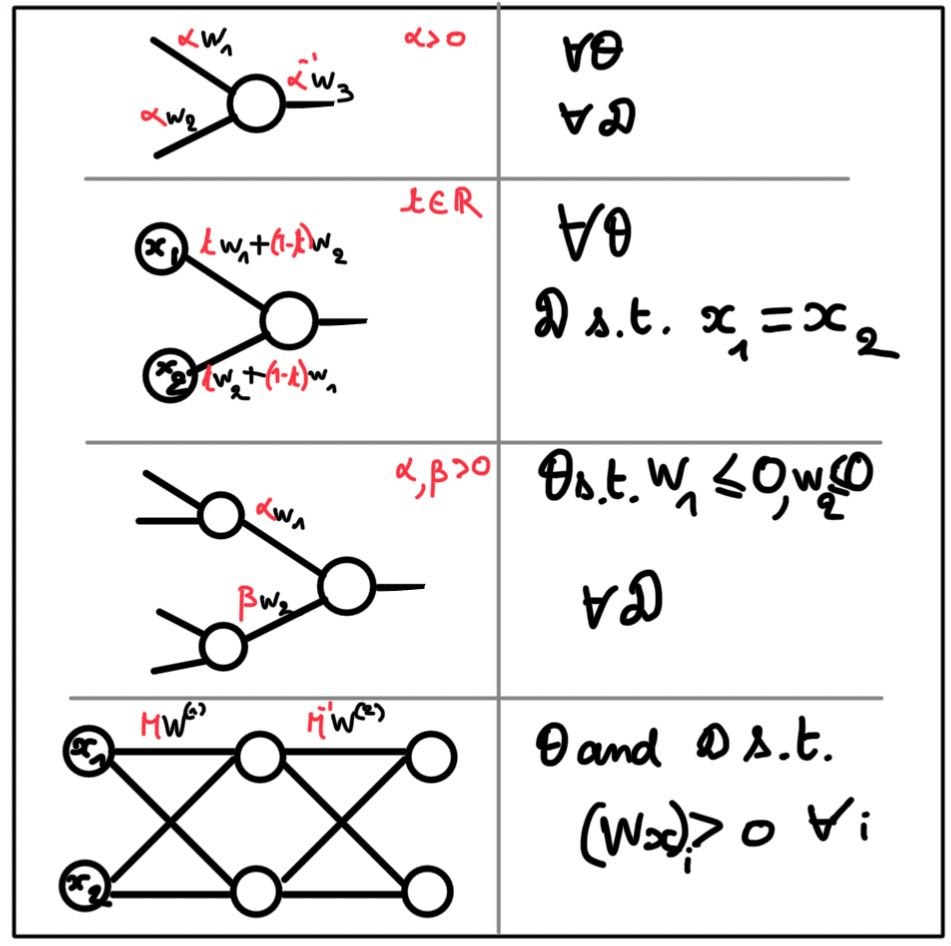
\includegraphics[width=0.33\linewidth]{images/draft/hierarchy-symmetries.jpg}
    \caption{From top to bottom:\textbf{(1.)} A rescaling symmetry is valid for all parameters and dataset. \textbf{(2.)} A shared input symmetry is valid at any neurons with equal inputs \textbf{(3.)} A dead ReLU symmetry is valid after layer $1$ for any neuron with all input parameter negative \textbf{(4.)} An active subspace symmetry is valid for parameter and data such that a set of neurons in a layer have positive only activations.\pnote{Last symmetry is harder to formalize: describe $M$}}
    \label{fig:hierarchy-symmetries}
\end{figure}

\myline

\paragraph{Data augmentation}
Data augmentation is a brute force approach in which a dataset is enriched with new samples crafted from original ones.
Note that a single continuous symmetry can generate infinitely many augmented points, so it is clear that the augmented dataset cannot be complete.
A drawback of data augmentation is the impact on storage and computational costs due to increase in data points.
In the symmetry discovery scenario, \cite{yang2023p4icml} reports better performances when using data augmentation generated from learned symmetries rather than pure equivariance to those learned symmetries even though for the ground truth symmetries, pure equivariance performs better.
Data augmentations may be the only game in town when the transformations are difficult to express with group theory (e.g. face recognition \cite{bhattacharya20192sicaccpi}), or to address example partial symmetry.
Instead of inferring symmetries as in symmetry discovery, some works propose to search directly for data augmentation policies with positive impact on the validation set \cite{cubuk20192iccvprc,lim2019anips}.
Data augmentation are often perceived as a cheap way to achieve invariance, less elegant than invariant architecture, but they have empirical success and are used frequently in industry.
\cite{shen2026} provides insight on the relevance of using equivariant architectures

\myline

\paragraph{Crafting invariant features}
Feature engineering, the goal is to featurize so that the featurization is invariant w.r.t. symmetries. However, this featurization might not be lossless, nor tailored to the specific need of the problem. Moreover one of the core strength of deep learning is learning representation, so doing featurization is doing by hand something that should be done by the model. 
\begin{itemize}
    \item random walk
    \item compute edge distances in geometric graphs
\end{itemize}

\myline

\paragraph{Predictable transformation}
Translate the input by one unit and rotate the output by a quarter. This is predictable but different from equivariance.
Or even in the case of scalar: move to the right by 1 unit and increase a scalar quantity by $C$ (constant) or move by 1 unit and multiply a quantity by $C$.

\myline

\paragraph{Interplay between invariance and equivariance in geometric deep learning}
A common scheme to build a globally invariant model is to stack equivariant layers and put an invariant layer at the end.

\myline

\paragraph{Symmetry to subsets of group, partial symmetry}
A relaxation discussed in \cite{romero2023} takes the form of achieving equivariance on a subset of a group (ex: rotations in [-90 degrees, +90 degrees] for face or on MNIST which has 6 and 9 potential confusion). This is particularly weird since the subset is not a group. This is also weird because a tilted 6 will not have the same range as a straight 6. \cite{romero2023} propose a way to have some layers fully equivariant and other layers partially equivariant.

\paragraph{Ranged symmetry} In this case, we would want to have symmetry over a specific range of transformations. For example for the MNIST dataset, we might ideally want symmetry to  some range of 2D rotations but not to the full 2D rotation group because otherwise digits 6 and 9 would be symmetries of each other. 

\paragraph{Small deformation} Consider a hand drawing. This drawing would still be recognizable even if it were drawn with some light tremors or instability. But if we apply the same "tremoring" operation again and again on the drawing, at some point it would not be considered the same anymore. This is another case of partial symmetry w.r.t. a transformation.

\myline

\paragraph{Derivative fields of geometric deep learning}
These derivative fields are less focused on symmetry.
\textit{Topological deep learning} is concerned with higher order message passing \cite{papillon2023,papamarkou2024}.
\textit{Categorical deep learning} seems to be concerned with programs and out of distribution generalization.

\myline

\paragraph{Geometric deep learning}
The objective of Geometric Deep Learning \cite{bronstein2017ispm, bronstein2021} is twofold: (1) provide a unifying view of deep learning architectures and (2) extend deep learning on new domains like graphs or manifolds in a convincing, principled way
In this field symmetry and equivariance are used a design principle.
This makes it possible to derive the form of a convolutional neural network from requiring translational equivariance, convolution is thus given a particular role.
\cite{kondor2018p3icml} argues that convolution is not just a way to achieve equivariance to a group action, it is also necessary necessary that an equivariant feedforward networks implements a (generalized group) convolution which takes the form 
\[
    (f\ast g)(u)=\int_Gf(uv^{-1})g(v)d\mu(v).
\]
The discrete counterpart of this equation for the correlation operation of functions having $K$ channels was introduced in \cite{cohen2016}, which reads by adapting notation to stay consistent with the above:
\[
    (f\star g)(u)=\sum_{v \in G}\sum_k^Kf_k(v)g_k(u^{-1}v).
\]
where $f$ and $g$ are functions on the group $G$.

\myline

\paragraph{Equivariant deep learning}
The field of equivariant deep learning can be seen as a subfield of Geometric Deep Learning focused on designing equivariant neural networks.
Diffusion models can be made equivariant: \cite{xu2026a} propose an architecture for molecular structure generation which constrains the target probability distribution to be SE(3)-equivariant.




\end{document}